% \documentclass[12p]{article}
\documentclass{article}
% bibliographystyle{seg asdf}
% \tiny\bibligoraphy{seq_eg} .bib file
% \usepackage[margin=1in, headheight=110pt]{geometry}
\usepackage[letterpaper, margin=1in]{geometry}
\usepackage{amssymb, amsmath, amsfonts, amsthm}
\usepackage{mathpazo}
\usepackage{setspace}
% \usepackage{probsoln}
\usepackage{fancyhdr}
\usepackage{hyperref}
\usepackage{float}
\usepackage{tikz}
\usepackage{enumitem}
\usepackage{listings}
% \usepackage{lipsum}
\usepackage{parskip} % Use for extra line spacing

\setlength{\parindent}{0 in}

% TODO change these when we figure them out
\newcommand{\namenobold}{Hover Wars}
\newcommand{\name}{\textbf{\namenobold}}
% Darkwire
% Flatlined
% Hot Steel
% Hover Wars    <--- James' pick
% Netrunners
% Last Stand
% Standoff
% Pulse
% Sector 6
% Silver Helix
% Street Warriors
\newcommand{\team}{Team A --- Pressurized Studios}
\newcommand{\botcount}{4}

\pagestyle{fancy}
\lhead{Final Product Design}
\rhead{CPSC 585 --- Winter 2019}

\lfoot{\namenobold{}}
\rfoot{\team{}}

\newenvironment{hangingpar}[1]
  {\begin{list}
          {}
          {\setlength{\itemindent}{-#1}%%'
           \setlength{\leftmargin}{#1}%%'
           \setlength{\itemsep}{0pt}%%'
           \setlength{\parsep}{\parskip}%%'
           \setlength{\topsep}{\parskip}%%'
           }
    \setlength{\parindent}{-#1}%%
    \item[]
  }
  {\end{list}}


\newcommand{\sep}{\;}
\newtheorem{theorem}{Theorem}
\theoremstyle{definition}
\newtheorem{definition}[theorem]{Definition}

\newcommand\floor[1]{\lfloor#1\rfloor}
\newcommand\ceil[1]{\lceil#1\rceil}
\begin{document}
\begin{titlepage}
  \begin{center}
    \vspace*{1cm}
    \Large{\textbf{University of Calgary}}\\
    \Large{\textbf{CPSC 585 --- Winter 2019 --- Games Programming}}\\
    \vfill
    \line(1,0){400}\\[1mm]
    \huge{\textbf{\namenobold{}}}\\
    \large{\textbf{Final Product Design Document}}\\
    \line(1,0){400}\\
    \vfill
    \Large{\textbf{\team{}}}\\
    \Large{Austin Easton, Evan Quan, James Cot\'{e}, Jianan Ding}\\
    \large{April 12, 2019}
    % \today \\
  \end{center}
\end{titlepage}
% \thispagestyle{fancy}
\setcounter{page}{0}
\tableofcontents
\pagenumbering{gobble}
\break{}
\pagenumbering{arabic}
% \onehalfspacing

\section{Introduction}

\begin{figure}[htpb]
  \centering
  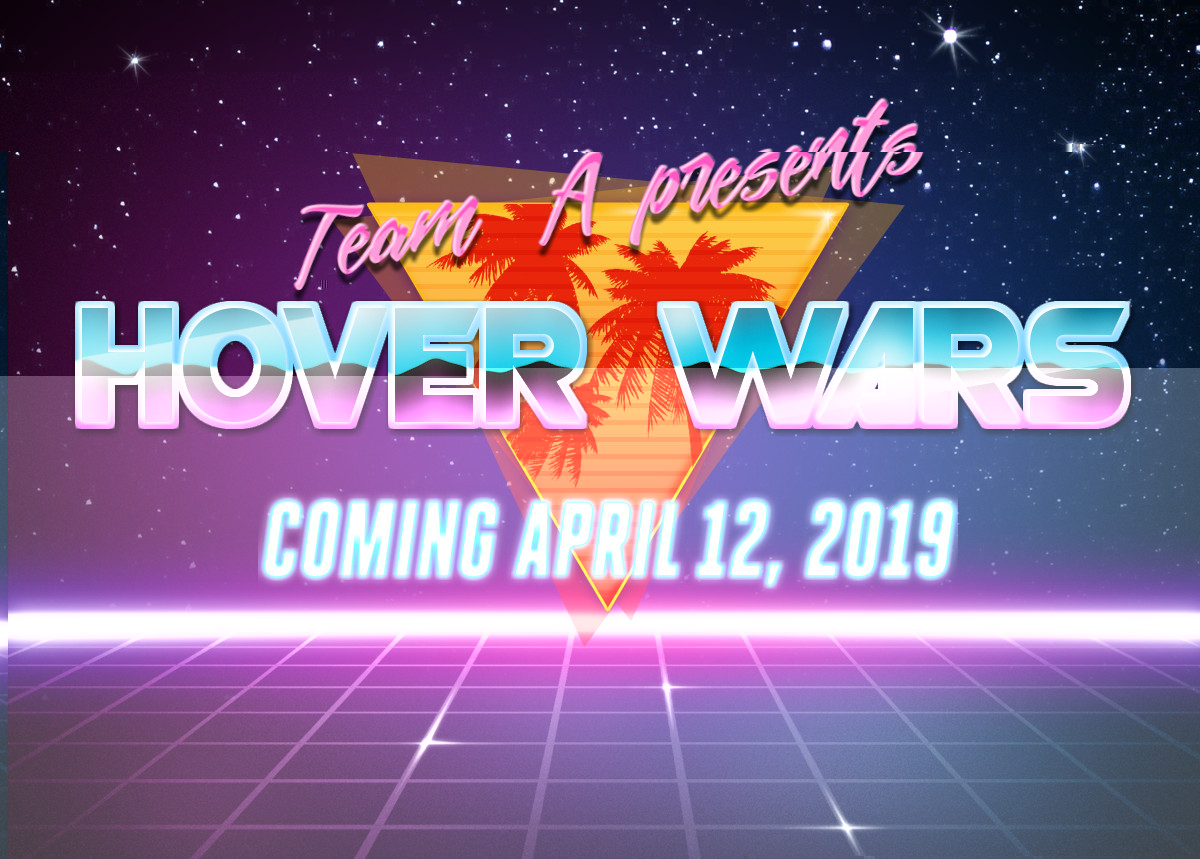
\includegraphics[width=1.0\linewidth]{images/title_art_hover_wars.jpg}
\label{fig:title_art}
\end{figure}

Over the course of the last couple of months, there have been a few design
decision changes. This document serves to highlight and discuss them.

\section{Gameplay}

\subsection{Game Modes}

The central game mode we propose to implement is \textbf{free-for-all}. At a lower
priority, other modes may be developed if enough time is available.

\subsubsection{Free-for-all}

Each game is composed of a single round that lasts for the duration of a timer.
Each player is placed in an arena to control a hovercraft with various
abilities. They must fight each other in a free-for-all battle with those
abilities, amidst a number of AI-controlled hovercrafts roaming the arena to
hunt down players.

The central goal of the game is to gain the highest score possible before the
round is over. Players have the following means to gain score:
\begin{itemize}
  \item Attacking other player hovercrafts, which can only be done in
    multiplayer. This can be through the use of abilities accessible to every
    player.
  \item Attacking AI-controller hovercrafts (bots), which can be done in both
    single and multiplayer. Bot hovercrafts do not have all the abilities of
    player hovercrafts and so reward less points.
  \item Picking up power-ups. These help the player gain points by improving
    their abilities, but also innately give points when they are picked up.
\end{itemize}

\subsection{Arenas/Maps}

% TODO

\textbf{Primary Environmental Features}

These are basic features that are core to the map's design, and so play a high
priority  in their implementation.

\begin{itemize}
  \item \textbf{Barriers/obstacles} --- These can block movement and
    projectiles. These can take the form of various things: street lamps,
    walls, buildings, tunnels, or other structures.
  \item \textbf{Ramps} --- Ramps lead to higher and lower platforms, or can be jumped
    off of over obstacles. This can provide better vision of certain parts of
    the map, give opportunities to jump between arenas.
\end{itemize}

\textbf{Tentative Environmental Features}

These features are open to be cut, either due to time constraints to implement
or potential game design problems they introduce.

\begin{itemize}
  \item \textbf{Speed pads} --- Driving over these will give a momentary boost of
    speed. Designed for getting power-ups quicker, and chasing or escaping
    other players.

    \textbf{Potential problem:} While these make sense for a racing game, they
    may detract from the gameplay for a combat arena game. Players will
    typically want full control over their vehicle and driving over a speed
    bump in locations where they don't want it can be annoying. If a temporary
    speed boost mechanic is to be implemented, it may be better to have a speed
    boost power-up instead of speed pads.
  \item \textbf{Pits} --- Falling into the pit will instantly destroy the player
    hovercraft. Avoid at all costs or try to bump enemies into it.

    \textbf{Potential problem:} Depending on the placement, size and frequency
    of the pit, players can be easily frustrated if they are constantly
    falling in it. Instant death mechanics such as this can also break the flow
    of gameplay.
  \item \textbf{Jump pads} --- Driving over these, will give a vertical boost
    while maintaining horizontal momentum. Designed for jumping over obstacles
    or reaching areas of higher elevation.

    \textbf{Potential problem:} Similar to speed pads, players may not
    actually want to use them when traversing across the map. It can
    potentially be very disorienting to players to use jump pads, especially if
    they lose control of their movement while in the air. Ramps can serve the
    same purpose without making the player lose control. Anohter possible
    solution would be to allow players to influence their trajectory while they
    are in the air.
\end{itemize}

It is important to note that more features doesn't always mean a better map.
Even if the idea of certain map features are cool or interesting on paper, if
they detract from the overall gameplay experience in practice, it is better to
leave them out. There is value in a good but simple map design.

\subsection{Hit Points, Lives, and Damage}

There are a few hit point and damage systems we have considered. We are
currently committed to implement the \textbf{hit and continue} system, but will
be open to change as we play-test.

\subsubsection{Hit and Continue}

Modelled after \textbf{Mario Kart}'s damage system, hovercrafts are blown away or
spun around when they are hit by abilities, temporarily making the player or
bot that was hit lose control of their vehicle. Shortly afterwards, control is
regained and the hovercraft is given a few seconds of invincibility before
continuing on playing. This minimizes the downtime during play since there is
no respawning, while still punishing players that get hit. It also avoids the
disorienting effect that respawning can have, especially if the map is not
familiar to the player.

\subsubsection{Lives with Hit Points}

Players start the game alive with a small set amount of hit points, which will
be explicitly displayed to the player. They can be damaged by the abilities of
other hovercrafts, lowering their current hit points. The same temporary loss
of control will occur as the hit and continue system. When all hit points are
removed, the player's hovercraft is destroyed.

When a player's hovercraft is destroyed, they are momentarily out of the game
before respawning randomly at one of the respawn points on the map. If another
player destroyed said hovercraft, that player is awarded points for the kill.

Under this system, bots could have fewer hit points than players.

\subsubsection{One Hit One Kill}

Similar to the lives and hit points system, but players are instantly destroyed
upon impact of an ability. This makes getting hit more punishing and further
promotes players to dodge abilities.

\subsection{Players}

\subsubsection{Movement}

\begin{itemize}
  \item \textbf{Acceleration/braking} --- This was deemed unnecessary as we have tuned the driving model so players can very easily stop and change directions at will.
  \item \textbf{Dashing} --- Dash charges were implemented so that players could consecuatively dash to their target to use spikes. Not only did this feel better than without the charge system, but it also improved the spike ability's usefulness.
\end{itemize}

\subsubsection{Abilities}

\begin{itemize}
  \item \textbf{Rocket} --- Initially we had a very short cooldown for the rocket.
  \item \textbf{Spikes} ---
  \item \textbf{Trail} ---
\end{itemize}

\subsection{Bots}

\subsubsection{Movement}

% TODO describe bot path behaviour in AI

\subsubsection{Abilities}

% TODO dashing?
More than promised, bots are able to use all abilities.

\begin{enumerate}
  \item \textbf{Rockets} ---
  \item \textbf{Dashing} --- Bots would be able to dash out of the way to dodge
    abilities.
  % \item \textbf{Trail} --- Bots will try to intercept the player's path to get
  %   them caught in the trail. This is
  % TODO explain trail behaviour
  % TODO explain spike behaviour
\end{enumerate}

\subsection{Power-Ups}


\subsubsection{Spawning}


\subsection{Menu}

\section{Game Design}

\subsection{Aesthetic}

We finally decided to follow an a 1980-theme retrofuturistic art and music style
commonly referred to as Outrun.

\begin{figure}[htpb]
  \centering
  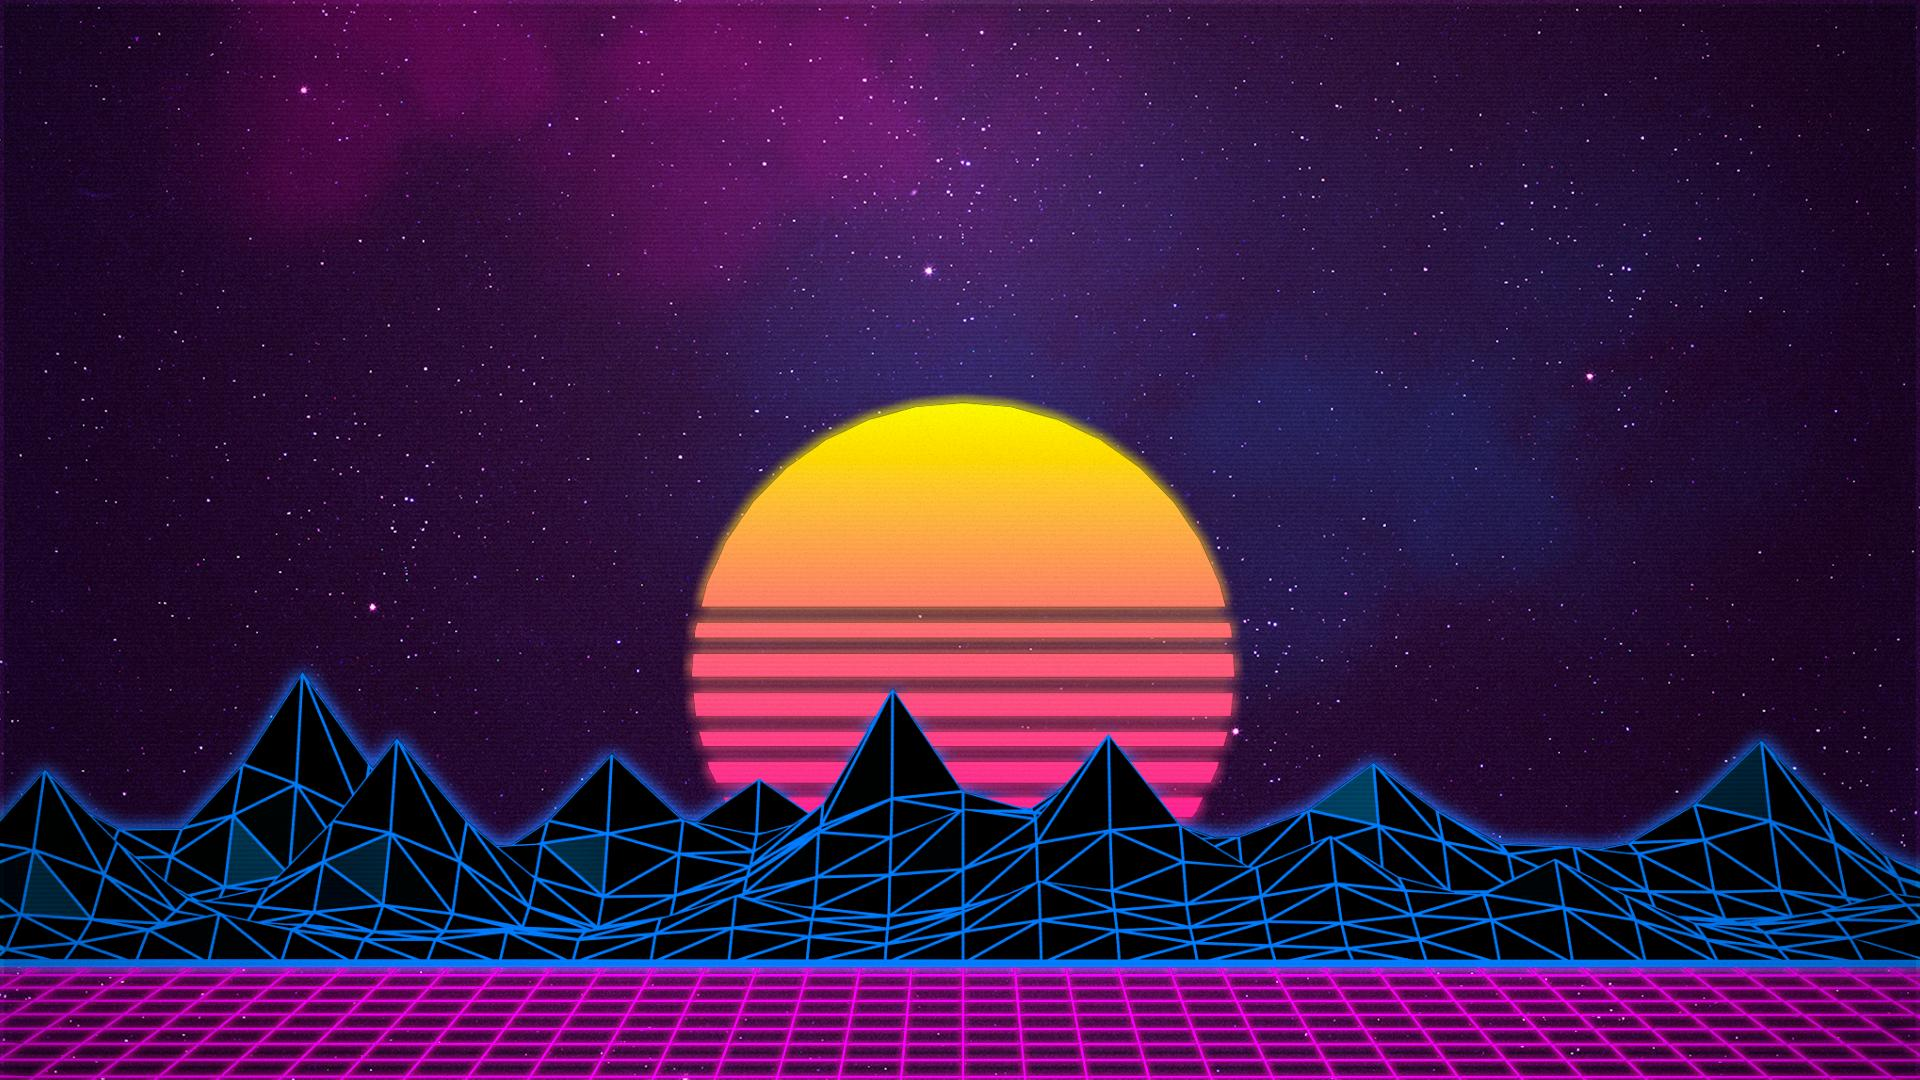
\includegraphics[width=0.8\linewidth]{images/art/main_menu4.jpg}
  \caption{Wireframe appearance. Bright neon colours contrast heavy use of black.}
\label{fig:theme01}
\end{figure}

\begin{figure}[htpb]
  \centering
  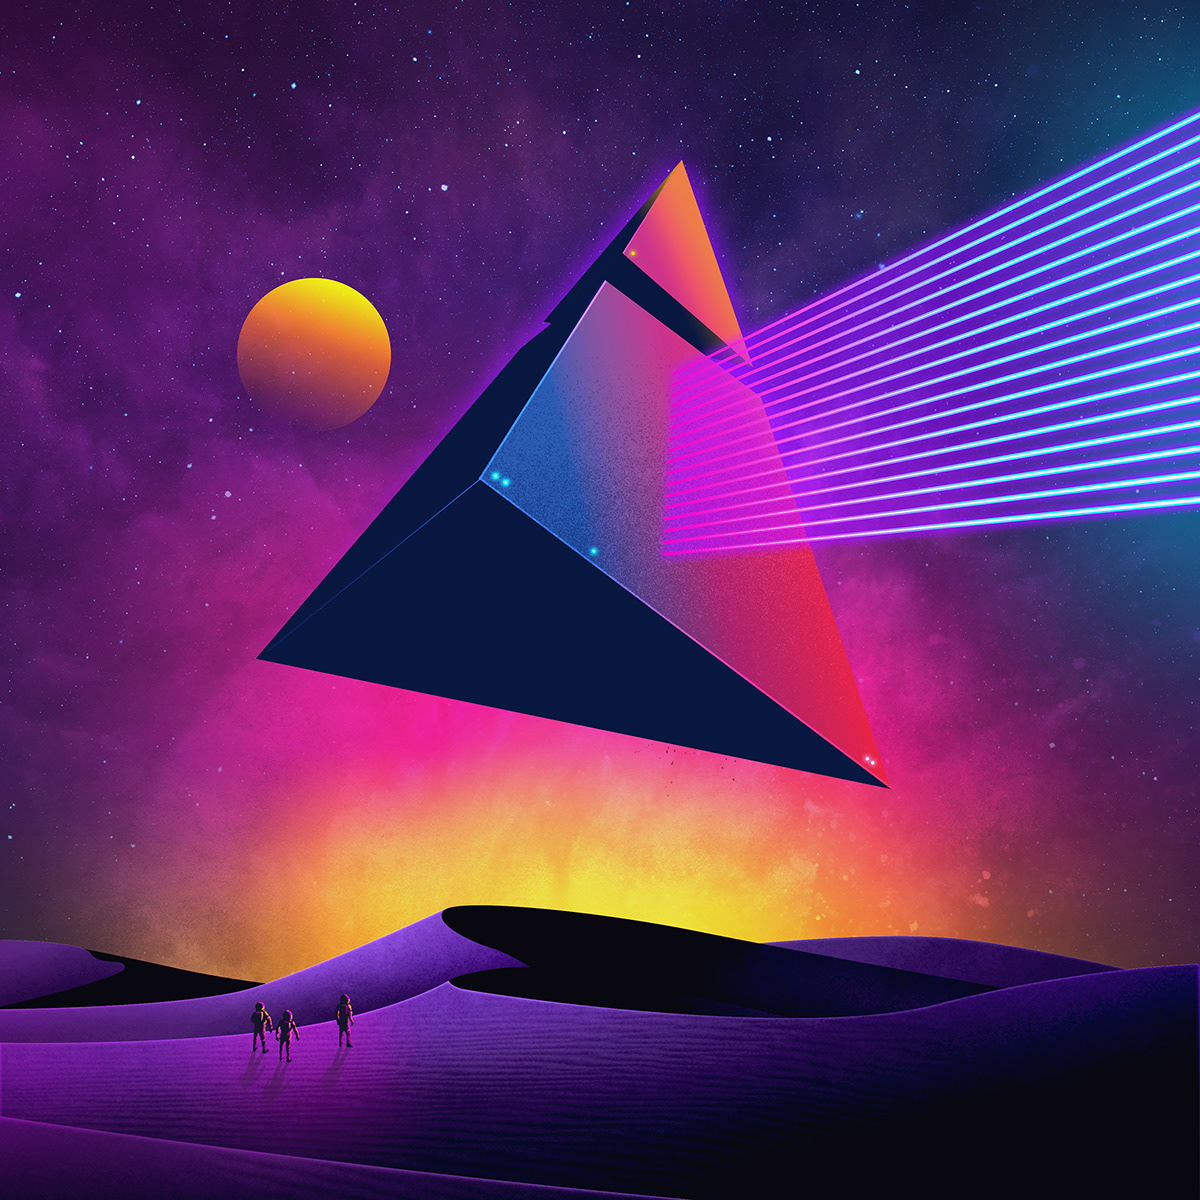
\includegraphics[width=0.8\linewidth]{images/art/start_menu4.jpg}
  \caption{}
\label{fig:theme02}
\end{figure}

\subsection{Designer Insight/Goals}

Looking back at our designer goals in our intial high-level design document, this is how we followed through:

\subsubsection{Role of AI}

The introduction of AI-controlled hovercrafts (bots) adds an interesting
element to the game, but also a few problems.

First, given our past experience and the time-frame creating the AI, we don't
believe the bots will be equally competent to a skilled human player. If bots
are given a hovercraft with equal capability to that of a player, it is
unlikely they will be able to utilize their abilities and movement sufficiently
to compete with players, or have sufficient game sense to outplay and counter
different play styles. This poses a problem for single-player, as competing
against a group of underperforming bots will not particularly fun or
challenging.

To address the challenge issue, it is possible to give bots point bonuses when
they score to improve their chances to beat players. However, this does not
necessarily address the fun issue, as the player will still experience fighting
against simple bots.

Instead, bots can be given an alternative role rather than replacing a player.
By explicitly giving them less capabilities than the player, and having them
exist in-game independent from the player count, they can add an extra depth to
the gameplay without heavily relying on the depth of their capabilities. The
benefit is that if the bots end up less capable than we initially planed, the
combat can still be just as fun since bots will be in greater numbers and team
up against the players. If they are more capable than we initially planned then
all the better, since this will simply make the gameplay more engaging.

Overall, the focus of multiplayer will be on the interactions between players
for the multiplayer experience, where the bots will provide a background or
secondary element to the gameplay. For single player, the bots will be core to
the gameplay, as they are the only enemy against the player.

\subsubsection{Driving System}

\subsubsection{Getting Hit}

Independent of which damage system we implement (hit and continue, lives with
hit points, or one hit one kill), we want to ensure that it is in line with
number of our design goals.
\begin{itemize}
  \item \textbf{Emphasize the impact of getting hit} ---
  \item \textbf{Ease user memory load} ---
  \item \textbf{Easy to Interpret} ---
\end{itemize}

\subsubsection{Abilities}

In designing our abilities, we have several goals in mind. For each one
included, we want to make sure that they:
\begin{itemize}
  \item \textbf{Feel distinct to use:}
  \item \textbf{Serve different purposes:}
  \item \textbf{Introduce some level of counterplay:}
  \item \textbf{Are deliberate in their use:}
\end{itemize}

\end{document}
